\documentclass[11pt,twoside,a4paper]{article}
%=========================== En-Tete =================================
%--- Insertion de paquetages (optionnel) ---
\usepackage{a4}	             % pour la taille   
\usepackage[T1]{fontenc}     % pour les font postscript
\usepackage{lmodern}
\usepackage{amsmath, amsthm} % tres bon mode mathematique
\usepackage{amsfonts,amssymb}% permet la definition des ensembles
\usepackage{float}           % pour le placement des figures
\usepackage{verbatim}

\usepackage{lastpage}

\usepackage{eso-pic} %% mettre une image de fond !!

\usepackage{tikz}
\usetikzlibrary{decorations.pathmorphing, shapes}

\usepackage{fontspec}
\defaultfontfeatures{Mapping=tex-text,Scale=MatchLowercase}
%% \setmainfont{Cyberpunk Is Not Dead}

\usepackage[top=2.0cm, bottom=2.0cm, left=2.0cm, right=2.0cm]{geometry}

\def\magazineTitle{The CyberPunk Gazette}

\usepackage{lipsum} 

\usepackage{multicol}

\usepackage{tikzpeople}

% % % en-tete et pieds de page configurables : fancyhdr.sty
\usepackage{fancyhdr}
\pagestyle{fancy}
\fancyhf{}
\fancyhead[LE,RO]{  }
\fancyfoot[LE]{\thepage /\pageref{LastPage} \hfill
	\textbf{\magazineTitle }
\hfill \includegraphics[width=0.5cm]{../../../../imgGraphics/logos/glider/logo-glider.png} }
\fancyfoot[RO]{\includegraphics[width=0.5cm]{../../../../imgGraphics/logos/glider/logo-glider.png} \hfill
	\textbf{\magazineTitle }
\hfill \thepage /\pageref{LastPage}}
\renewcommand{\headrulewidth}{0.0pt}
\renewcommand{\footrulewidth}{0.5pt}
\addtolength{\headheight}{0.5pt}
\fancypagestyle{plain}{
	\fancyhead{}
	\fancyfoot{}
	\renewcommand{\headrulewidth}{0pt}
}

%--- Definitions de nouvelles commandes ---

\def\peopleOnRight{% 
	
\begin{tikzpicture}
		\node[criminal,evil,saturated,shield,sword,minimum size=0.75cm]{};
	\end{tikzpicture}
}

\def\peopleOnLeft{% 
	
\begin{tikzpicture}
		\node[nun,female,good,mirrored,monitor,saturated,shield,sword,minimum size=0.75cm]{};
	\end{tikzpicture}
}

%--- Pour le titre ---
\def\date{\today}
\def\maketitle{%
	\setlength{\parindent}{0em}
	\begin{center}
		\begin{tabular}[c]{c|c|c}
			\peopleOnRight						& \setmainfont{Chomsky} \Huge{ \magazineTitle }				&	\peopleOnLeft							\\
												& 															&											\\
			Issue 0, Volume 0 					& \setmainfont{DS Zierschrift} \Large{Neo-Paris News}		& \date										\\
												& 															&											\\
	\setmainfont{FoglihtenDeH02} \textbf{G-z}	& \setmainfont{FoglihtenDeH02} \textbf{T+++++2+++++t}		& \setmainfont{FoglihtenDeH02} \textbf{Z-G}	\\
		\end{tabular}~\\
	\end{center}
	\setlength{\parindent}{2\parskip}
}%

\usepackage{hyperref}
%% http://www.andy-roberts.net/writing/latex/pdfs -- for some properties...
%% https://tex.stackexchange.com/questions/26529/how-can-i-generate-pdf-metadata-from-latex
\hypersetup{
	pdfauthor={Gaby Wald / Gabriel Chandesris},
	pdftitle={\magazineTitle "News Generator" \today},
	pdfsubject={\magazineTitle "News Generator" \today},
	pdfkeywords={\magazineTitle "News Generator" \today},
	pdfproducer={PDFLaTeX (production)},
	pdfcreator={PDFLaTeX (creation)}
	%% urlcolor=green,
}
%% https://tex.stackexchange.com/questions/79395/option-clash-for-hyperref-package

%============================= Corps =================================
\begin{document}

\AddToShipoutPicture{
    \AtPageUpperLeft{1cm}{
		\put(0,0){
			\parbox[b][\paperheight]{\paperwidth}{%
			\includegraphics[width=\paperwidth]{../../../../imgGraphics/cyberpunk/CyberPunkRedBandeauHaut.jpg}%
			\vfill
		}}}
    
    %% \AtPageCenter{ AtPageCenter }
    %% \AtTextCenter{ AtTextCenter }
    %% \AtStockCenter{ AtStockCenter }
    
    \AtTextCenter{ 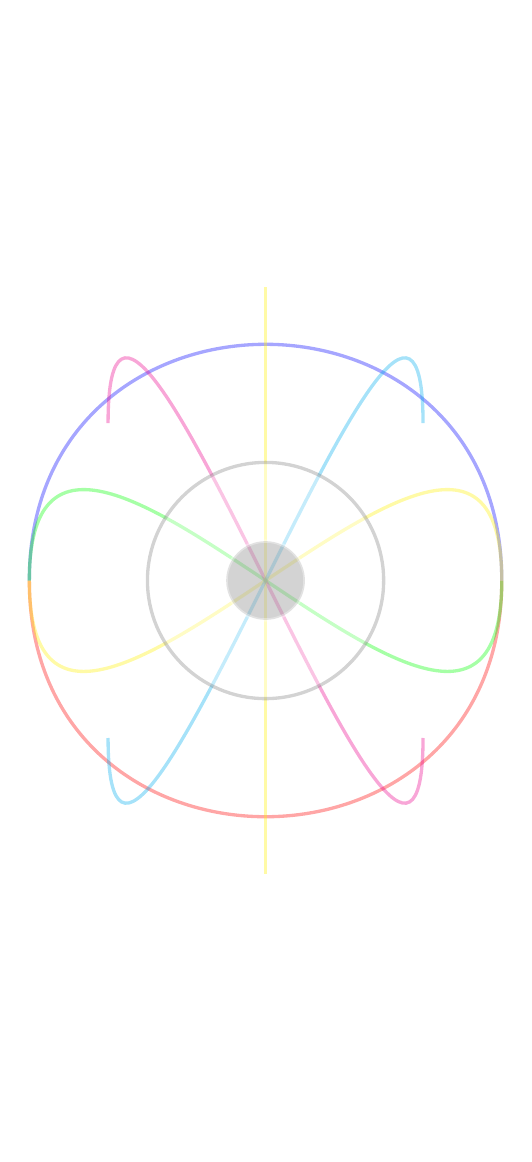
\begin{tikzpicture}[opacity=0.35, scale=2.00] %% ,shift={(0.00,-5.00)}] %% ,rotate=-90] 
    	%% ,xshift=-12]
    	%% ,xshift=-12,yshift=-12]
    	%% ,shift={(12,12)}]
		%% \draw [very thin, gray] (-3,-3) grid (3,3);
		\draw [very thick, blue   ] (-1.50, 0.00) ..controls +(0, 2) and +(0, 2).. ( 1.50, 0.00);
		\draw [very thick, red    ] (-1.50, 0.00) ..controls +(0,-2) and +(0,-2).. ( 1.50, 0.00);
		\draw [very thick, green  ] (-1.50, 0.00) ..controls +(0, 2) and +(0,-2).. ( 1.50, 0.00);
		\draw [very thick, magenta] (-1.00, 1.00) ..controls +(0, 2) and +(0,-2).. ( 1.00,-1.00);
		\draw [very thick, yellow ] ( 0.00, 1.50) ..controls +(0, 2) and +(0,-2).. ( 0.00,-1.50);
		\draw [very thick, yellow ] (-1.50, 0.00) ..controls +(0,-2) and +(0, 2).. ( 1.50, 0.00);
		\draw [very thick, cyan   ] ( 1.00, 1.00) ..controls +(0, 2) and +(0,-2).. (-1.00,-1.00);
		\draw [very thick, gray, fill=white] (0.00,0.00) circle (0.75);
		\draw [very thick, white, fill=gray] (0.00,0.00) circle (0.25);
	\end{tikzpicture} }
    
    \AtPageLowerLeft{1cm}{\includegraphics[width=\paperwidth]{../../../../imgGraphics/cyberpunk/CyberPunkRedBandeauBas.jpg}}
}

% ecrire le titre...
\maketitle


\LARGE{\centering \setmainfont{Sprawl} Gigaquads of scientific data copied by hacker}

\begin{multicols}{2}

\small

{\centering \Huge \setmainfont{FoglihtenDeH02} \textbf{Q+\_9\_+q} }~\\

\textbf{}~\\
\emph{'COMPANYNAME' discovered this morning that a massive quantity of computer data had been stolen from one of their Central Mainframes.}~\\
The stolen files contained data from a massive scientific research program, which 'COMPANYNAME' had been working on for the past 3 years.
 Around TOTALFILESIZE Gigaquads of data was copied before the intruder disconnected.
'COMPANYNAME' will undoubtedly try to discover the corporation behind this theft.

~\\

\vfill~\vfill

\textbf{Computer failure blaimed for research loss}~\\
\emph{}~\\
'COMPANYNAME' again found themselves in trouble as gigaquds of data where wiped from their system. In a statement today the company claimed it had evidence that the files where deliberately deleted by a malicious hacker.~\\
The data deleted was the combined results of a large scale scientific test, being conducted by 'COMPANYNAME' in order to develop new technology.
In a statement today the company said that serious damage had been done and that it could cost the company millions of dollars to perform the research again.

~\\

\vfill~\vfill

\textbf{Major corporation suffers complete data loss}~\\
\emph{}~\\
'COMPANYNAME' are today boosting their security systems as their file servers suffered yet another complete failure. The company has come under attack on several occasions in the last month by hackers who have yet to be identified.~\\
The company found that masses of corporate data has been destroyed.
It is not known how much this will cost the company but there is little doubt that serious damage has been done. This level of data loss could not occur without serious repurcusions.

~\\

\vfill~\columnbreak

%% {\small \lipsum[1-3] }~\\

{\centering \Huge \setmainfont{FoglihtenDeH02} \textbf{\{1=:=!\}} }~\\

\begin{multicols}{2}

\textbf{Specific Article 1}~\\

\emph{Catchphrase Lorem Ipsum}~\\

\lipsum[5-7]~\\

\end{multicols}

{\centering \rule{0.34\textwidth}{1pt} }~\\

Automatic Generated Page. \textsc{Not real news !}~\\
\emph{News Generator} by \textbf{Gaby Wald}~\\

\end{multicols}

\input{../latexTemplates/template_journal_footer.tex}

